\chapter{Referencial teórico}

\section{Moscamed, a instituição e a técnica}

A Biofábrica Moscamed Brasil é uma organização social situada no Vale do São Francisco, mais precisamente em Juazeiro-BA, responsável pelo controle biológico e monitoramento ambientalmente seguro de pragas em culturas de alto interesse econômico, tais como, manga, uva, melão, maçã, papaia, goiaba e acerola \cite{MOSCAMED2010LINHAS}. Bem como o controle do vetor transmissor de doenças mais importante para a saúde pública atualmente, o mosquito \textit{Aedes Aegypt} \cite{MOSCAMEDINST2003, MOSCAMED2010LINHAS}.

A organização possui atividades em larga escala voltadas para a produção e liberação na natureza de insetos estéreis modificados, via raios-X no caso da mosca-das-frutas e via alteração genética no caso do Mosquito-da-dengue. Possui o planejamento de produção/liberação de 200 (duzentos) milhões de machos estéreis por semana \cite{MOSCAMEDINST2003, MOSCAMED2003CTI}. Ademais, realiza capacitação, treinamento e disseminação de informações técnico-científicas de sua área de atuação para a comunidade \cite{MOSCAMED2010AREAS}.

O controle e monitoramento é realizado através da TIE em ambas as linhas de produção. Concebida em 1937, por Edward F. Knipling, a TIE é considerada um tipo de controle autocida ou genético, visto que a praga é utilizada em seu próprio controle \cite{TIE2015}. Os insetos estéreis são produzidos e liberados em quantidades bem maiores do que as encontradas na natureza, competem pelo acasalamento com os selvagens e acabam copulando com as fêmeas. As fêmeas, por sua vez, no caso das moscas, realizam a postura de ovos não fecundados. Já no caso dos mosquitos, o gene modificado repassado para as próximas gerações elimina ou inviabiliza as fêmeas adultas. As duas maneiras fazem com que a geração posterior de insetos tenha sua população reduzida. A repetição deste processo continuamente garante a manutenção do baixo índice populacional e em alguns casos leva à erradicação \cite{MOSCAMEDINST2003, MOSCAMED2003CTI, MOSCAMED2010LINHAS}.

Segundo \citeonline{TIE2015}, até 1970 o controle de insetos era efetuado por meio de métodos baseados na utilização de inseticidas químicos sintéticos. O uso dos inseticidas sofreu diversas restrições durante a década de 70, à partir de então popularizou-se o conceito de Manejo Integrado de Pragas (MIP), onde diferentes ferramentas de controle (como por exemplo produtos químicos, agentes biológicos, ferômonios, dentre outras) são integradas de maneira planejada e coerente. A TIE foi posteriormente incorporada aos programas de MIP em grandes áreas, pois se trata de uma técnica de controle biológico onde as ações não são diretamente executadas por um produtor e sim por uma coordenação regional gestora do programa. A TIE supre, em sua maioria, a necessidade de tratamento com inseticidas no combate às pragas, promovendo a redução das despesas de produção e o aumento consequente da qualidade final e da segurança alimentar do produto agrícola \cite{MOSCAMED2003CTI}.

Cerca de 28 países estão aplicando a TIE em larga escala para supressão populacional e erradicação em locais como a Ásia, ilhas do Pacífico, Oceania, África, Europa e alguns países das Américas e Caribe. No Brasil, 11 estados são beneficiados pela TIE por intermédio da coordenação da Moscamed juntamente ao Ministério da Agricultura, Pecuária e Abastecimento e das Agências estaduais de Defesa Agropecuária. São os estados da Bahia, Pernambuco, Ceará, Rio Grande do Norte, Piauí, Paraíba, Sergipe, Minas Gerais, Espírito Santo, Rio Grande do Sul e Santa Catarina \cite{MOSCAMEDINST2003, MOSCAMED2003CTI}.


\section{A estação meteorológica e a influência das condições climáticas nas espécies controladas pela Moscamed}

As estações meteorológicas surgiram com a finalidade de suprir a necessidade de medir variáveis climáticas. O estudo dessas variáveis é de grande valia para as atividades humanas, pois implica de forma direta ou indireta no atual modelo de desenvolvimento, visto que uma política de desenvolvimento sustentável necessita de monitoramento sobre os recursos naturais finitos fortemente relacionados ao clima. No Brasil, inicialmente, a obtenção e avaliação de dados meteorológicos coletados era feita por intermédio do Instituto Nacional de Meteorologia - INMET. Esse processo possuía uma amostragem relativamente pequena e estava sujeita à erros humanos \cite{torres2015aquisicao}.
  
O crescimento tecnológico proporcionou a possibilidade da criação de estações meteorológicas automáticas que abrem mão da interferência humana, prevenindo assim a ocorrência de erros e além disso incrementam consideravelmente o desempenho, praticidade e confiabilidade das medições realizadas \cite{torres2015aquisicao}.  

A estação meteorológica \textit{Vantage Vue™} (figura \ref{img:estacao}) é uma estação automática \textit{wireless} composta de dois módulos, sendo o primeiro deles um conjunto de sensores (figura \ref{img:sensores}) e o segundo um console (figura \ref{img:console}). A suíte de sensores é alimentada por energia solar, inclui uma bateria reserva e contém os seguintes sensores: coletor de chuva, sensor de umidade/temperatura, anemômetro e sensor de direção do vento. Após a coleta de dados pelos sensores, os mesmos são atualizados e enviados via rádio de baixa potência para o console \cite{SITEDAVIS, VVINSTMANUAL}.

\newpage

\begin{figure}[!htb]
\centering
    \caption{\label{img:estacao} A estação meteorológica \textit{Vantage Vue™}}
    \subcaptionbox{\label{img:sensores} Suíte de sensores}{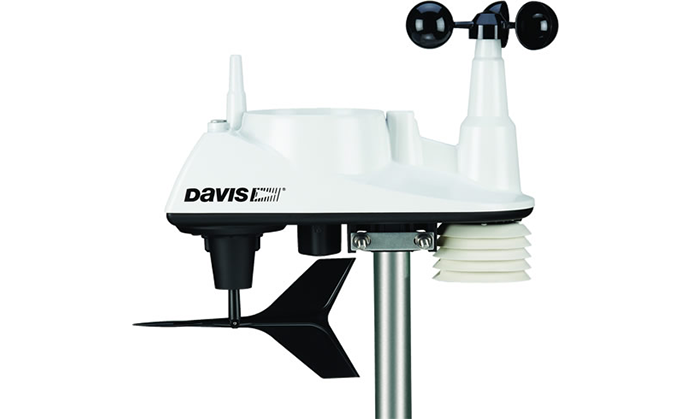
\includegraphics[scale=.26]{img/vantagevue}}\qquad
    \subcaptionbox{\label{img:console} Console}
{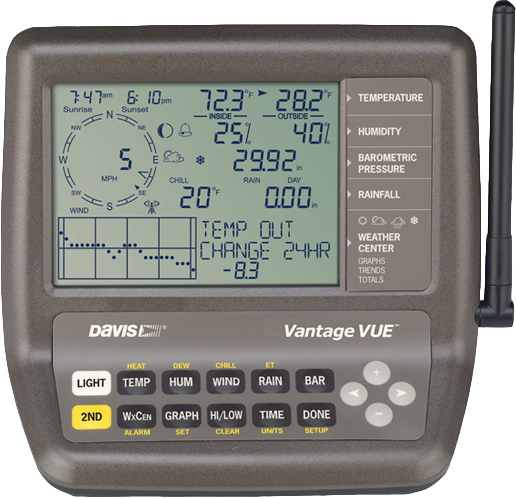
\includegraphics[scale=.21]{img/console}}
    \legend{\textbf{Fonte:} \citeonline{SITEDAVIS}}
\label{fig:dag}
\end{figure}

Por sua vez, o console \textit{Vantage Vue™} é responsável pela exibição e registro dos dados de sua estação. Possui também a opção de interação com computador via módulo \textit{ethernet} vendido separadamente, \textit{WeatherLinkIP}® (figura \ref{img:weatherlinkip}) \cite{SITEDAVIS, VVCINSTMANUAL}.

\imagem{0.57}{weatherlinkip}{O \textit{datalogger WeatherLinkIP®}}{O autor}
\newpage

O módulo \textit{WeatherLinkIP}® consiste de um \textit{datalogger} que conecta o console da estação à internet. O módulo transfere os dados climáticos obtidos do console para o computador, com a finalidade gerar uma base de dados permanente. As principais variáveis exportadas e arquivadas pelo \textit{datalogger} são a hora/data da medição, temperatura interna e externa, direção e velocidade do vento, precipitação e a umidade interna e externa \cite{WLIP}.

O tamanho da memória não volátil do módulo é de 128KB. A memória é preenchida de acordo com o intervalo (em minutos) de atualização definido pelo usuário. Portanto, o período de tempo ao qual as amostras se referem pode ter uma extensão maior ou menor. Por exemplo, caso o usuário escolha a taxa de atualização de um e um minuto, o módulo terá espaço suficiente para armazenar dados de cerca de quarenta e duas horas. Por outro lado, se a frequência de atualização for de trinta minutos, o armazenamento terá dados de cinquenta e três dias \cite{WLIP}.

\subsection{A influência do clima na mosca-das-frutas}

A mosca-das-frutas é um inseto que sofre diversas alterações em seu ciclo de vida de acordo com as mudanças climáticas. Por volta de 250 (duzentas e cinquenta) espécies dessas pragas atacam variedades de plantas frutíferas de grande interesse econômico. São insetos da ordem \textit{Diptera} e família \textit{Tephritidae}. Estão presentes em todo território brasileiro, porém existem dois gêneros com importância maior, sendo uma originária das Américas Central e do Sul e outra cuja a introdução no país ocorreu no início do século XX, os gêneros \textit{Anastrepha} e \textit{Ceratitis}, respectivamente. Na Região do Vale do Submédio São Francisco há 11 (onze) espécies de \textit{Anastrepha} já identificadas \cite{paranhos2008moscas}.

Os ciclos de vida de ambos os gêneros supracitados são semelhantes, diferencia\-ndo-se apenas na questão do tempo de desenvolvimento das fases. O ciclo se inicia com a oviposição realizada pela fêmea nos frutos, após a eclosão a larva penetra no endocarpo e depois deixam o fruto para empupar no solo e por fim emergirem como adultos \cite{paranhos2008moscas}.
  
Segundo \citeonline{calore2013fatores}, em um estudo relacionado aos insetos de goiaba, a sazonalidade dos elementos climáticos/meteorológicos têm influência direta ou indireta sobre esses insetos. Diretamente, os elementos do clima podem atuar na mortalidade ou no desenvolvimento dos insetos, alterando a oviposição, alimentação, crescimento, desenvolvimento e migração. Os aspectos climáticos podem atuar de forma indireta pela influência na atividade dos inimigos naturais dos insetos e pela variação na qualidade dos recursos disponíveis devido as mudanças fisiológicas e bioquímicas na planta hospedeira.

Ainda de acordo com \citeonline{calore2013fatores}, as variáveis meteorológicas que estão mais relacionadas com a dinâmica populacional de insetos e diversos ecossistemas são a temperatura, a umidade relativa, a precipitação pluviométrica e a velocidade do vento. Em algumas espécies a evaporação, a insolação e o fotoperíodo também são importantes.

Em relação a mosca-das-frutas têm-se a temperatura do ar como principal influenciador no desenvolvimento de suas fases de ovo, larva e adulta, enquanto a temperatura do solo é predominante na fase de pupa \cite{garcia1998influencia}. Por exemplo, em situações de temperaturas superiores a 35ºC ou inferiores a 10ºC não há desenvolvimento de nenhuma das fases do ciclo de vida da mosca-da-fruta da espécie \textit{Anastrepha fraterculus} \cite{araujo2008levantamento}. Além disso, em regiões semiáridas a precipitação, as temperaturas elevadas e a disponibilidade de hospedeiros regem os picos populacionais da mosca-das-frutas da espécie citada, pois a precipitação ocasiona o aumento da umidade no solo, viabilizando o desenvolvimento da fase de pupa, que em sua maioria ocorre numa camada contemplada pelos dez primeiros centímetros do solo. Essa camada é altamente vulnerável ao dessecamento e portanto pode causar a inviabilidade das pupas e dificultar a emergência dos adultos devido ao solo ressecado \cite{calore2013fatores, araujo2008levantamento}.

\subsection{A influência do clima no mosquito-da-dengue}

De forma análoga à mosca-das-frutas, os mosquitos \textit{Aedes Aegypti} também sofrem variações em seu ciclo vital e em seu comportamento mediante modificações climáticas. De acordo com \citeonline{hopp2001global}, o aumento da temperatura global e outras mudanças climáticas podem modificar a área geográfica de presença desse inseto. Como por exemplo na Colômbia, onde os insetos eram limitados pela altitude de 1500 metros devido ao intenso frio e hoje em dia são encontrados em níveis acima de 2200 metros em razão da elevação da temperatura.
 
A temperatura e a precipitação pluviométrica, apresentam grande significância em relação ao desenvolvimento e sobrevivência dessa espécie, como pode ser observado na figura \ref{img:aedeslc} \cite{hopp2001global, ribeiro2006associaccao}. 

Ainda na figura \ref{img:aedeslc}, em algumas fases estão destacadas as faixas de valores das variáveis que são cruciais para o desenvolvimento e/ou sobrevivência do inseto, em outras etapas destaca-se apenas a dependência de determinados fatores. Na incubação por exemplo (transição entre a fase de ovo e a fase de larva), necessita-se da temperatura igual ou superior a 13ºC e uma lâmina d’água de pelo menos 10 milímetros de espessura. Em outro caso, na fase de pupa o desenvolvimento do inseto é sensível à temperatura média diária. As faixas de temperaturas aqui ilustradas são referentes à taxa de sobrevivência igual a 1 (um), como pode ser visualizado na figura \ref{img:survivor}.

%\newpage

\imagem{0.54}{aedeslc}{O Ciclo de Vida do Mosquito \textit{Aedes Aegypti} e suas dependências climáticas diárias}{\citeonline{hopp2001global} (Adaptado) }
 
\imagem{0.55}{survivor}{Dependência da temperatura na sobrevivência dos estágios de vida do mosquito \textit{Aedes Aegypti}}{\citeonline{hopp2001global}(Adaptado) }

De acordo com \citeonline{depradine2004climatological}, uma elevada pressão de vapor de água facilita a atividade dos mosquitos, tornando suas atividades de alimentação ou ataque mais frequentes, provocando a propagação acentuada da doença.

Além do ciclo de vida do mosquito, a dinâmica de casos de doenças relacionadas ao vetor também flutua com as condições do clima. A flutuação está diretamente ligada ao aumento de temperatura, pluviosidade e umidade do ar, pois o conjunto desses fatores favorecem o crescimento da quantidade de criadouros disponíveis e o desenvolvimento do vetor \cite{ribeiro2006associaccao}.

\section{Sistema Operacional Android}

O \textit{Android} é a plataforma de desenvolvimento \textit{mobile} mais popular do mundo, está presente em mais de 190 países e possui centenas de milhões de dispositivos ativos. A plataforma conta com a contribuição da comunidade \textit{open-source} Linux e mais de 300 parceiros em \textit{hardware}, \textit{software} e operadoras. A plataforma permite a criação de aplicativos por meio da linguagem de programação Java. A Google, dententora da plataforma, disponibiliza o Kit de Desenvolvimento de Software (\textit{Software Development Kit - SDK}) e o Ambiente de Desenvolvimento Integrado (IDE) para a criação de aplicativos nativos para \textit{Android} \cite{SITEANDROID}.

\subsection{Características e Arquitetura}

A pilha de software da plataforma \textit{Android} possui código aberto e é baseada em Linux, conforme ilustrada pela figura \ref{img:Android2}. A escolha do Linux como base da pilha é justificada pela utilização de recursos de segurança, outras atividades de gerenciamento de \textit{hardware} já disponíveis nesse sistema operacional e pela facilidade proporcionada aos fabricantes no desenvolvimento de \textit{drivers} de \textit{hardware} para um \textit{kernel} conhecido \cite{SITEANDROID, gandhewar2010google}.

\imagem{0.72}{Android2}{A pilha de software do Android}{\citeonline{SITEANDROID2} (Traduzido)}

A segunda camada, abstração de \textit{hardware} (\textit{Hardware Abstration Layer - HAL}), é responsável por fornecer para a interface de programação de aplicação (\textit{Application Programming Interface - API}) Java o acesso aos componentes de \textit{hardware}, tais como o módulo de câmera ou \textit{bluetooth}. O \textit{Android Runtime - ART} é capaz de executar para cada aplicativo uma máquina virtual própria que requer poucos recursos, possibilitando a execução de vários aplicativos simultaneamente. Os dois últimos componentes e alguns serviços são implementados em código nativo que utiliza bibliotecas em C/C++, porém essas funcionalidades podem ser acessadas através de APIs Java \cite{SITEANDROID}.

O sistema operacional fornece seus recursos por intermédio de APIs programadas em linguagem Java. As APIs compõem os blocos necessários para a criação dos aplicativos, como o sistema de visualização e os gerenciadores de recursos, notificações e atividades \cite{SITEANDROID}.

Na camada mais alta têm-se os aplicativos padrão do sistema que podem ser utilizados para prover funcionalidade à outros aplicativos de terceiros, eliminando a necessidade de desenvolver novamente uma funcionalidade, por exemplo o envio de uma mensagem de texto ou a captura de uma fotografia \cite{SITEANDROID, saha2008developer}.

\section{Aplicações Web}

O grande sucesso da \textit{Web} como arquitetura para desenvolvimento de aplicações pessoais, sociais e de negócios tem impulsionado os desenvolvedores à criarem novas aplicações ou portar \textit{softwares} existentes para a \textit{Web} \cite{fraternali1998conceptual}. A numerosidade das aplicações desenvolvidas fez nascer a necessidade de estabelecer padrões/princípios para o desenvolvimento de aplicações \textit{Web} \cite{pressman2000tangled}.
   
A engenharia de software de desenvolvimento \textit{Web} possui pontos semelhantes e diferentes em relação à de \textit{software} convencionais. É semelhante pelo fato de buscar a realização de uma aplicação correta e completa, mediante os requisitos propostos, e difere porque deve considerar a arquitetura \textit{Web} para sua execução \cite{conte2005processos}.

As aplicações \textit{Web} podem ser divididas em duas categorias, aplicações hipermídia \textit{Web} e aplicações de \textit{software Web}. A primeira é uma aplicação não-convencional onde as informações são disseminadas através de nós, \textit{links}, âncoras, estruturas de acesso e é disponibilizada na \textit{Web}. As tecnologias utilizadas comumente para desenvolver essas aplicações são o \textit{HyperText Markup Language - HTML}, JavaScript e pacotes de multimídia. As aplicações de \textit{software Web} são aplicações nos modelos tradicionais que dependem da arquitetura \textit{Web} para seu funcionamento, tais como sistemas legados de banco de dados, bases de conhecimento, \textit{e-commerce}, entre outros \cite{mendes2005investigating}.

A elaboração de aplicações \textit{Web} deve considerar três dimensões em sua concepção, são elas:

\begin{itemize}
	\item Estrutural: diz respeito a organização das informações e seus relacionamentos semânticos.
	\item Navegacional: como o nome já diz, representa a forma como as informações organizadas pela camada Estrutural serão acessadas.
	\item Apresentação: é a forma como as informações e a aparência dadas à ela serão expostas ao usuário.
\end{itemize}

A qualidade da navegação e da apresentação são tão importantes quanto a qualidade da informação em si \cite{fraternali1998conceptual}. O principal objetivo da engenharia de software \textit{Web} é que haja o desenvolvimento correto da aplicação em termos de estrutura, funcionalidades, aspectos navegacionais e interação com o usuário \cite{pastor2004fitting}.

\section{Aplicações Multiplataformas}

O desenvolvimento de aplicativos multiplataformas consiste em gerar aplicações para diversos sistemas operacionais e para \textit{Web} à partir de um único código fonte. Essa forma de desenvolver ganha mais popularidade à cada dia, principalmente devido ao fato de algumas ferramentas permitirem a utilização de linguagens de programação bastante conhecidas pela comunidade, tais como o HTML, JavaScript e o \textit{Cascading Style Sheet (CSS)}. O código nativo de cada sistema operacional é mascarado por chamadas à APIs, realizadas apenas quando se deseja operar sobre um dispositivo, como câmera ou giroscópio \cite{raj2012study, palmieri2012comparison, dalmasso2013survey}.

Devido ao fato de se possuir apenas uma base de código, a manutenibilidade do software se torna bem menos custosa do que prover soluções nativas específicas para cada plataforma \cite{raj2012study}. \citeonline{palmieri2012comparison} destacam alguns pontos positivos relacionados ao desenvolvimento de aplicações com esse tipo de ferramenta:

\begin{itemize}
\item Redução das habilidades requeridas aos programadores;
\item Redução do tamanho do código;
\item Redução do tempo de desenvolvimento e custos de manutenção a longo prazo;
\item Redução de conhecimento necessário sobre às APIs nativas;
\item Maior facilidade de desenvolvimento;
\item Incremento da participação no mercado.
\end{itemize}


Aplicações \textit{cross-platform} podem ser classificadas em quatro tipos de abordagem, \textit{Web}, Híbrida, Interpretada e Compilação Cruzada. A abordagem \textit{Web} classifica aplicações cuja execução é feita no navegador do dispositivo móvel e os dados são providos por um servidor, neste caso nenhuma instalação é realizada no armazenamento do aparelho. A metodologia Híbrida requer instalação e também usa o navegador do aparelho para renderizar e mostrar as telas da aplicação, porém existe a possibilidade de efetuar chamadas às APIs JavaScript com a finalidade de operar sobre o \textit{hardware} do aparelho \cite{raj2012study, dalmasso2013survey}.

As aplicações interpretadas, como o próprio nome já diz, têm seu código interpretado em tempo de execução por um interpretador. Assim como as aplicações Híbridas, possuem uma camada de abstração que provê o acesso ao \textit{hardware} via APIs. No caso da Compilação Cruzada, o código fonte é convertido para os códigos binários nativos de cada plataforma e o \textit{hardware} é acessado pelas APIs nativas de cada sistema \cite{raj2012study}.

Existem prós e contras em cada tipo de abordagem, portanto deve-se adotar a que mais se adequa ao projeto a ser desenvolvido. Por exemplo, a abordagem \textit{Web} não possui acesso aos sensores do aparelho \textit{mobile}, já a abordagem Híbrida possui performance inferior em relação as aplicações nativas, pois são executadas no navegador. Enquanto isso, na metodologia de Compilação Cruzada, códigos específicos de cada plataforma não podem ser reutilizados, como interface, acesso à localização e notificações \cite{raj2012study}.

A seleção da metodologia ideal depende majoritariamente dos requerimentos da aplicação. A tabela \ref{tab:crossplatform} mostra em uma escala de valores, quais abordagens são ideais para cada tipo de aplicação: 1 – Não preferível, 2 – Preferível, mas não é a metodologia ideal e 3 – Metodologia perfeita \cite{raj2012study}.

\begin{table}[!htb]
	\centering
	\caption{\label{tab:crossplatform} Tipos de aplicações e abordagens preferenciais.}
	\begin{adjustbox}{max width=\textwidth}
		\begin{tabular}{@{} p{5cm} ccc @{}}
		\toprule
		\textbf{Código da Aplicação} & \textbf{Web} & \textbf{Híbrida} & \textbf{Interpretada / Compilação Cruzada} \\ \hline

		\textbf{Aplicações baseadas em dados providos por um servidor} &
			3 & 2 & 1
		\\ \hline

		\textbf{Aplicações independentes} & 1 & 2 & 3\\ \hline

		\textbf{Aplicações baseadas em sensores e processamento de dados no dispositivo} & 1 & 2 & 3\\ \hline

		\textbf{Aplicações baseadas em sensores e processamento de dados no servidor} & 1 & 3 & 2\\ \hline

		\textbf{Aplicações Cliente-Servidor} & 1 & 3 & 2 \\ \bottomrule
	\end{tabular}
	\end{adjustbox}
	\legend{\textbf{Fonte:} \citeonline{raj2012study} (Traduzido)}
\end{table}


\section{API RESTful}
O estilo de arquitetura REST (\textit{Representational State Transfer}) consiste da utilização dos verbos do protocolo HTTP para representar ações no acesso à recursos identificados por um URI (\textit{Uniform Resource Identifier}). As comunicações realizadas com o estilo REST são \textit{stateless}, ou seja, os dados de uma requisição antiga não são repassados para uma requisição posterior. Portanto, é necessário o envio de todas as informações a cada nova requisição. As respostas enviadas pela API ao cliente possuem o formato JSON (\textit{Javascript Object Notation}) ou XML (\textit{Extensible Markup Language}) independentemente da representação original do recurso \cite{arcuri2017restful, fielding2000architectural}.

Os verbos HTTP utilizados comumente nesse tipo de arquitetura são o GET, POST, PUT e DELETE. As aplicações dos verbos estão exemplificadas na tabela \ref{tab:httpverbs} abaixo.

\begin{table}[!htb]
	\centering
	\caption{\label{tab:httpverbs} Métodos HTTP.}
	\begin{adjustbox}{max width=\textwidth}
		\begin{tabular}{@{} p{4cm} c p{10cm} @{}}
		\toprule
		\textbf{Método HTTP} & \textbf{Ação} & \textbf{Notas} \\ \hline

		\textbf{GET} &
			Ler & Recupera um recurso. \newline Exemplo: GET /livros/1 (recupera o recurso de identificador 1) \newline GET /livros (recupera vários recursos) \\ \hline

		\textbf{POST} & Criar & Cria um recurso com os parâmetros repassados. \newline Exemplo: POST /livros {“nomeLivro” : “nome”} 
\\ \hline

		\textbf{PUT} & Atualizar & Atualiza ou cria (caso não exista) um recurso identificado, com os valores repassados. \newline Exemplo: PUT /livros/1 {“nomeLivro” : “novoNome”}
\\ \hline

		\textbf{DELETE} & Deletar & Deleta um recurso identificado. \newline Exemplo: DELETE /livros/1 (deleta o recurso de identificador 1)
 \\ \bottomrule
	\end{tabular}
	\end{adjustbox}
	\legend{\textbf{Fonte:} \citeonline{hsieh2016method} (Traduzido)}
\end{table}

\section{Socket TCP}
O protocolo TCP (\textit{Transmission Control Protocol}) trabalha entregando os pacotes recebidos aos respectivos protocolos de aplicação atribuídos às portas de destino. Por exemplo, ao receber um pacote destinado à porta 80, os dados são entregues ao protocolo HTTP \cite{torres2001completo}.

Porém, quando mais de uma aplicação de mesmo tipo estão comunicando-se com a rede é necessário o uso de um \textit{socket} para definir uma conexão diferente para cada aplicação dentro de uma porta. Os \textit{sockets} gerados quando o transmissor e o receptor criam uma conexão, são definidos em duas classes, ativo e passivo. O primeiro é aquele que envia dados, enquanto o segundo é aquele que recebe dados \cite{torres2001completo}.

As aplicações comunicam-se escrevendo e lendo de seus respectivos \textit{sockets}, ou seja, um \textit{socket} é a interface entre a camada de aplicação e a de transporte dentro de uma máquina como ilustra a figura \ref{img:tcpsocket} \cite{james2005redes}.

\imagem{0.75}{tcpsocket}{Processos de aplicação, \textit{sockets} e protocolo de transporte subjacente}{\citeonline{james2005redes}}